%%%%%%%%%%%%%%
%% Run LaTeX on this file several times to get Table of Contents,
%% cross-references, and citations.

%% If you have font problems, you may edit the w-bookps.sty file
%% to customize the font names to match those on your system.

%% w-bksamp.tex. Current Version: Feb 16, 2012
%%%%%%%%%%%%%%%%%%%%%%%%%%%%%%%%%%%%%%%%%%%%%%%%%%%%%%%%%%%%%%%%
%
%  Sample file for
%  Wiley Book Style, Design No.: SD 001B, 7x10
%  Wiley Book Style, Design No.: SD 004B, 6x9
%
%
%  Prepared by Amy Hendrickson, TeXnology Inc.
%  http://www.texnology.com
%%%%%%%%%%%%%%%%%%%%%%%%%%%%%%%%%%%%%%%%%%%%%%%%%%%%%%%%%%%%%%%%

%%%%%%%%%%%%%
% 7x10
%\documentclass{wileySev}

% 6x9
\documentclass{wileySix}

\usepackage{graphicx}
\usepackage{listings}

\usepackage{color}
 
\definecolor{codegreen}{rgb}{0,0.6,0}
\definecolor{codegray}{rgb}{0.5,0.5,0.5}
\definecolor{codepurple}{rgb}{0.58,0,0.82}
\definecolor{backcolour}{rgb}{0.95,0.95,0.92}
 
\lstdefinestyle{mystyle}{
    backgroundcolor=\color{backcolour},   
    commentstyle=\color{codegreen},
    keywordstyle=\color{magenta},
    numberstyle=\tiny\color{codegray},
    stringstyle=\color{codepurple},
    basicstyle=\footnotesize,
    breakatwhitespace=false,         
    breaklines=true,                 
    captionpos=b,                    
    keepspaces=true,                 
    numbers=left,                    
    numbersep=5pt,                  
    showspaces=false,                
    showstringspaces=false,
    showtabs=false,                  
    tabsize=2,
    language=sh
}
 
\lstset{style=mystyle}

%%%%%%%
%% for times math: However, this package disables bold math (!)
%% \mathbf{x} will still work, but you will not have bold math
%% in section heads or chapter titles. If you don't use math
%% in those environments, mathptmx might be a good choice.

% \usepackage{mathptmx}

% For PostScript text
\usepackage{w-bookps}

%%%%%%%%%%%%%%%%%%%%%%%%%%%%%%%%%%%%%%%%%%%%%%%%%%%%%%%%%%%%%%%%
%% Other packages you might want to use:

% for chapter bibliography made with BibTeX
% \usepackage{chapterbib}

% for multiple indices
% \usepackage{multind}

% for answers to problems
% \usepackage{answers}

%%%%%%%%%%%%%%%%%%%%%%%%%%%%%%
%% Change options here if you want:
%%
%% How many levels of section head would you like numbered?
%% 0= no section numbers, 1= section, 2= subsection, 3= subsubsection
%%==>>
\setcounter{secnumdepth}{3}

%% How many levels of section head would you like to appear in the
%% Table of Contents?
%% 0= chapter titles, 1= section titles, 2= subsection titles, 
%% 3= subsubsection titles.
%%==>>
\setcounter{tocdepth}{2}

%% Cropmarks? good for final page makeup
%% \docropmarks

%%%%%%%%%%%%%%%%%%%%%%%%%%%%%%
%
% DRAFT
%
% Uncomment to get double spacing between lines, current date and time
% printed at bottom of page.
% \draft
% (If you want to keep tables from becoming double spaced also uncomment
% this):
% \renewcommand{\arraystretch}{0.6}
%%%%%%%%%%%%%%%%%%%%%%%%%%%%%%

%%%%%%% Demo of section head containing sample macro:
%% To get a macro to expand correctly in a section head, with upper and
%% lower case math, put the definition and set the box 
%% before \begin{document}, so that when it appears in the 
%% table of contents it will also work:

\newcommand{\VT}[1]{\ensuremath{{V_{T#1}}}}

%% use a box to expand the macro before we put it into the section head:

\newbox\sectsavebox
\setbox\sectsavebox=\hbox{\boldmath\VT{xyz}}

%%%%%%%%%%%%%%%%% End Demo


\begin{document}


\booktitle{Cerdas Menguasai Python}
\subtitle{Dalam 24 Jam}

\authors{Rolly M. Awangga\\
\affil{Informatics Research Center}
%Floyd J. Fowler, Jr.\\
%\affil{University of New Mexico}
}

\offprintinfo{Cerdas Menguasai Python, First Edition}{Rolly M. Awangga}

%% Can use \\ if title, and edition are too wide, ie,
%% \offprintinfo{Survey Methodology,\\ Second Edition}{Robert M. Groves}

%%%%%%%%%%%%%%%%%%%%%%%%%%%%%%
%% 
\halftitlepage

\titlepage


\begin{copyrightpage}{2019}
%Survey Methodology / Robert M. Groves . . . [et al.].
%\       p. cm.---(Wiley series in survey methodology)
%\    ``Wiley-Interscience."
%\    Includes bibliographical references and index.
%\    ISBN 0-471-48348-6 (pbk.)
%\    1. Surveys---Methodology.  2. Social 
%\  sciences---Research---Statistical methods.  I. Groves, Robert M.  II. %
%Series.\\
%
%HA31.2.S873 2007
%001.4'33---dc22                                             2004044064
\end{copyrightpage}

\dedication{`Jika Kamu tidak dapat menahan lelahnya belajar, 
Maka kamu harus sanggup menahan perihnya Kebodohan.'
~Imam Syafi'i~}

\begin{contributors}
\name{Rolly Maulana Awangga,} Informatics Research Center., Politeknik Pos Indonesia, Bandung,
Indonesia



\end{contributors}

\contentsinbrief
\tableofcontents
\listoffigures
\listoftables
\lstlistoflistings


\begin{foreword}
Sepatah kata dari Kaprodi, Kabag Kemahasiswaan dan Mahasiswa
\end{foreword}

\begin{preface}
Buku ini diciptakan bagi yang awam dengan git sekalipun.

\prefaceauthor{R. M. Awangga}
\where{Bandung, Jawa Barat\\
Februari, 2019}
\end{preface}


\begin{acknowledgments}
Terima kasih atas semua masukan dari para mahasiswa agar bisa membuat buku ini 
lebih baik dan lebih mudah dimengerti.

Terima kasih ini juga ditujukan khusus untuk team IRC yang 
telah fokus untuk belajar dan memahami bagaimana buku ini mendampingi proses 
Intership.
\authorinitials{R. M. A.}
\end{acknowledgments}

\begin{acronyms}
\acro{ACGIH}{American Conference of Governmental Industrial Hygienists}
\acro{AEC}{Atomic Energy Commission}
\acro{OSHA}{Occupational Health and Safety Commission}
\acro{SAMA}{Scientific Apparatus Makers Association}
\end{acronyms}

\begin{glossary}
\term{git}Merupakan manajemen sumber kode yang dibuat oleh linus torvald.

\term{bash}Merupakan bahasa sistem operasi berbasiskan *NIX.

\term{linux}Sistem operasi berbasis sumber kode terbuka yang dibuat oleh Linus Torvald
\end{glossary}

\begin{symbols}
\term{A}Amplitude

\term{\hbox{\&}}Propositional logic symbol 

\term{a}Filter Coefficient

\bigskip

\term{\mathcal{B}}Number of Beats
\end{symbols}

\begin{introduction}

%% optional, but if you want to list author:

\introauthor{Rolly Maulana Awangga, S.T., M.T.}
{Informatics Research Center\\
Bandung, Jawa Barat, Indonesia}

Pada era disruptif  \index{disruptif}\index{disruptif!modern} 
saat ini. git merupakan sebuah kebutuhan dalam sebuah organisasi pengembangan perangkat lunak.
Buku ini diharapkan bisa menjadi penghantar para programmer, analis, IT Operation dan Project Manajer.
Dalam melakukan implementasi git pada diri dan organisasinya.

Rumusnya cuman sebagai contoh aja biar keren\cite{awangga2018sampeu}.

\begin{equation}
ABC {\cal DEF} \alpha\beta\Gamma\Delta\sum^{abc}_{def}
\end{equation}

\end{introduction}

%%%%%%%%%%%%%%%%%%Isi Buku_

\chapter{Chapter 1}
\section{Chapter 1 | D. Irga B. Naufal Fakhri D4 TI 2C}
\subsection{Sejarah Python}
	Python adalah bahasa pemrograman interpretatif multiguna dengan filosofi perancangan yang berfokus pada tingkat keterbacaan kode. Python diklaim sebagai bahasa yang menggabungkan kapabilitas, kemampuan, dengan sintaksis kode yang sangat jelas,dan dilengkapi dengan fungsionalitas pustaka standar yang besar serta komprehensif. 

	Python diciptakan oleh Guido van Rossum di Scitchting Mathematisch Centrum (CWI) di Belanda pada tahun 1990-an. Bahasa python terinspirasi dari bahasa pemrograman ABC dan merupakan kelanjutan dari bahasa tersebut. Nama python sendiri bukan berasal dari nama ular python namun karena Guido adalah penggemar grup komedi Inggris bernama Monty Python. Guido masih menjadi penulis utama untuk python, walaupun python bersifat open source sehingga ribuan orang juga berkontribusi dalam mengembangkan python.

	Di tahun 1995, Guido melanjutkan pembuatan python di Corporation for National Research Initiative (CNRI) di Virginia Amerika, dimana dia merilis beberapa versi dari python.
Pada Mei 2000, Guido dan tim Python pindah ke BeOpen.com dan membentuk tim BeOpen PythonLabs. Di bulan Oktober pada tahun yang sama, tim python pindah ke Digital Creation (sekarang menjadi Perusahaan Zope). Pada tahun 2001, dibentuklah Organisasi Python yaitu Python Software Foundation (PSF). PSF merupakan organisasi nirlaba yang dibuat khusus untuk semua hal yang berkaitan dengan hak intelektual Python. Perusahaan Zope menjadi anggota sponsor dari PSF.

\subsection{Tanggal Rilis Python}
Semua versi python yang dirilis bersifat open source. Dalam sejarahnya, hampir semua rilis python menggunakan lisensi GFL-compatible. Berikut adalah versi major dan minor python berikut tanggal rilisnya.
\begin{itemize}
  \item Python 1.0 – Januari 1994
  \item Python 1.2 – 10 April 1995
  \item Python 1.3 – 12 Oktober 1995
  \item Python 1.4 – 25 Oktober 1996
  \item Python 1.5 – 31 Desember 1997
  \item Python 1.6 – 5 September 2000
  \item Python 2.0 – 16 Oktober 2000
  \item Python 2.1 – 17 April 2001
  \item Python 2.2 – 21 Desember 2001
  \item Python 2.3 – 29 Juli 2003
  \item Python 2.4 – 30 Nopember 2004
  \item Python 2.5 – 19 September 2006
  \item Python 2.6 – 1 Oktober 2008
  \item Python 2.7 – 3 Juli 2010
  \item Python 3.0 – 3 Desember 2008
  \item Python 3.1 – 27 Juni 2009
  \item Python 3.2 – 20 Februari 2011
  \item Python 3.3 – 29 September 2012
  \item Python 3.4 – 16 Maret 2014
  \item Python 3.5 – 13 September 2015
  \item Python 3.6 – 23 Desember 2016
\end{itemize}

\subsection{Perbedaan Python 2 dengan Python 3}
Pada Python 2 dan Python 3 memiliki kesamaan kapabilitas namun cara penggunaannya berbeda
\begin{itemize}
\item Print
\end{itemize}
Pada python2, print lebih seperti statement daripada fungsi
\begin{lstlisting}
print "Saya Belajar Python"
\end{lstlisting}
sedangkan pada python3, print digunakan sebagai fungsi
\begin{lstlisting}
print("Saya Belajar Python")
\end{lstlisting}

\begin{itemize}
\item Pembagian pada Interger
\end{itemize}
Pada Python 2, semua tipe data angka yang tidak mengandung desimal akan diperlakukan sebagai integer. Terlihat mudah pada awalnya, ketika mencoba untuk membagi kedua integer akan didapatkan tipe data float.

\begin{lstlisting}
3 / 2 = 1.5
\end{lstlisting}

Python 2 menggunakan floor division atau dibulatkan ke nilai paling rendah misalnya 1.5 jadi 1, 2.6 jadi 2 dan seterusnya. Pada Python 2.7 akan menjadi seperti ini:

\begin{lstlisting}
3
4
x = 3 / 2
print a
#Output
1
\end{lstlisting}

Untuk desimal maka tambahkan .0 setelah bilangan dan menjadi seperti ini 3.0 / 2.0  untuk mendapatkan hasil 1.5
Pada Python 3, pembagian pada bilangan integer lebih intuitif:

\begin{lstlisting}
a = 3 / 2
print(a)
#Output
1.5
\end{lstlisting}

Kita juga masih bisa melakukan 3.0 / 2.0  untuk mendapatkan 1.5 namun untuk mendapatkan floor division maka pada Python 3 gunakan //:
\begin{lstlisting}
b = 3 // 2
print(b)
#Output
1
\end{lstlisting}
Fitur pada Python 3 ini tidak bisa digunakan pada Python 2.7

\begin{itemize}
\item Dukungan Unicode
\end{itemize}

Ketika bahasa pemrograman menangani tipe data string (yang mana merupakan sekumpulan karakter), mereka bisa melakukan beberapa cara berbeda sehingga komputer dapat mengubah angka ke huruf dan simbol lain. Python 2 menggunakan alfabet ASCII secara default, sehingga ketika kita mengetik "Halo!"  maka Python 2 menangani string sebagai ASCII. Terbatas pada beberapa ratus karakter, ASCII mungkin bukan pilihan yang fleksibel untuk menangani proses encoding terutama yang non English.

Untuk menggunakan unicode yang lebih luwes, mendukung lebih dari 128,000 karakter maka kita harus mengetik u"Halo!" , dengan tambahan u  di depannya yang mana berarti Unicode.

Python 3 menggunakan Unicode secara default, yang mana menyelamatkan programmer dari tambahan kode lagi, lebih hemat waktu dan mudah untuk diisikan dan ditampilkan. Karena Unicode mendukung berbagai karakter linguistik yang beragam termasuk menampilkan emoji, penggunaan karakter secara default dengan encoding memastikan perangkat mobile didukung oleh program yang kita buat.

Jika kita ingin kode Python 3 kita mendukung Python 2, tambahkan u di depan string.

\subsection{Penggunaan Python di perusahaan dunia}
\begin{enumerate}
  \item Google adalah perusahaan besar yang menggunakan banyak kode Python di dalam mesin pencarinya. Dan mesin pencari google adalah yang paling terkenal di dunia.
  \item Youtube, situs video terbesar dan terpopuler di dunia, sebagian besar kodenya ditulis dalam bahasa Python.
  \item Facebook, media sosial terbesar di dunia, menggunakan Tornado, sebuah framework Python untuk menampilkan timeline.
  \item Instagram, siapa yang tidak kenal. Instagram menggunakan Django, framework python sebagai mesin pengolah sisi server dari aplikasinya.
  \item Pinterest, banyak menggunakan python untuk membangun aplikasinya.
  \item Dropbox, barangkali Anda adalah salah seorang pengguna layanan ini. Dropbox menggunakan python baik di sisi server maupun di sisi pengguna layanannya.
  \item Quora, salah satu situs tanya jawab terbesar di dunia, dibangun menggunakan Python.
  \item NASA, badan antariksa Amerika ini menggunakan Python untuk bidang sainsnya.
  \item NSA, badan mata – mata Amerika banyak menggunakan Python untuk analisa kriptografi dan intelijen
  \item Blender, Maya, software pembuat animasi 3D terkenal, menggunakan Python sebagai salah satu bahasa skrip pemrogramannya.
  \item Raspberry Pi, komputer mini yang banyak digunakan sebagai mikrokontroller, menggunakan Python sebagai bahasa utamanya.
  \item ESRI, produsen terkenal pembuat software pemetaan GIS banyak menggunakan Python di produknya.
\end{enumerate}
Untuk lebih lengkapnya bisa mengunjungi www.python.org/about/success/



\subsection{Cara menginstall Anaconda}
\begin{enumerate}
  \item Pastikan anda telah menginstall python dan anda mengetahui versi dari python yang telah anda install
  \item Download Anaconda dari website www.anaconda.com/distribution
  \item pilih sesuai dengan versi python anda, jika versi anda python3 maka pilih python3
  \item Setelah itu buka file yang telah anda download
  \item Setelah muncul gambar dibawah ini, tekan next
\begin{figure}[!htbp]
  \centering
  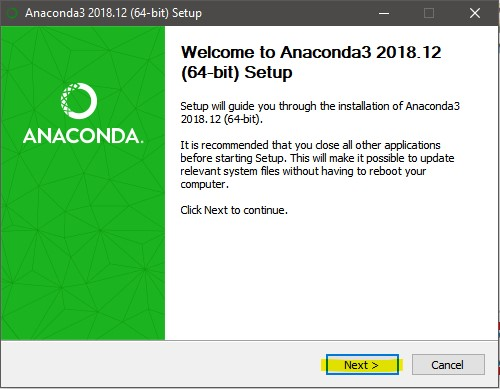
\includegraphics[height=3cm]{chapters/gambar/install1.jpg}
  \caption{Tampilan Instalasi 1}
\end{figure}

  \item Baca license agreement lalu tekan 'I Agree'
\begin{figure}[!htbp]
  \centering
  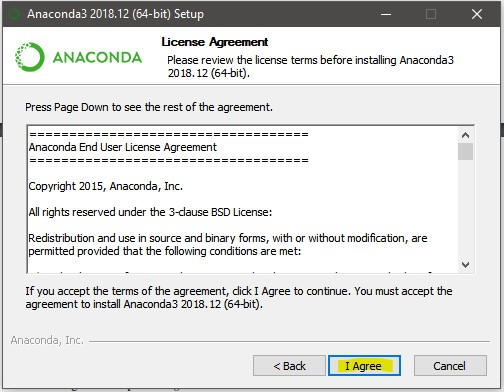
\includegraphics[height=3cm]{chapters/gambar/install2.jpg}
  \caption{Tampilan Instalasi 2}
\end{figure}

  \item Setelah itu pilih mau diinstall pada user yang sedang anda pakai atau kesemua user, direkomendasikan untuk memilih just me yaitu hanya user yang sedang dipakai saja
\begin{figure}[!htbp]
  \centering
  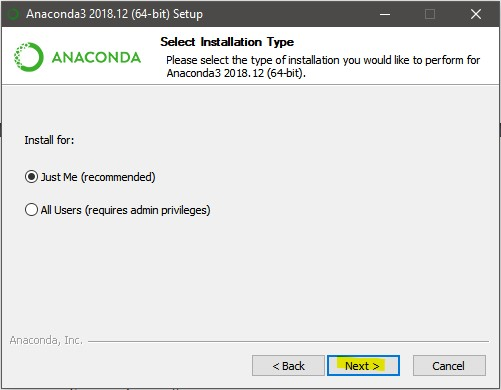
\includegraphics[height=3cm]{chapters/gambar/install3.jpg}
  \caption{Tampilan Instalasi 3}
\end{figure}

  \item Catat tempat dimana anda akan menginstall anaconda, lalu tekan 'Next'
\begin{figure}[!htbp]
  \centering
  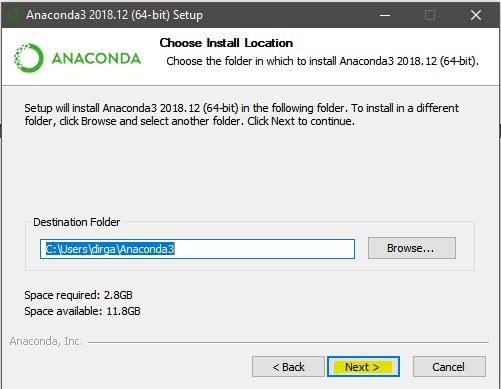
\includegraphics[height=3cm]{chapters/gambar/install4.jpg}
  \caption{Tampilan Instalasi 4}
\end{figure}

  \item Setelah itu anda diberi pilihan, direkomendasikan untuk tidak mengubah pilihan tersebut, lalu tekan 'Install'
\begin{figure}[!htbp]
  \centering
  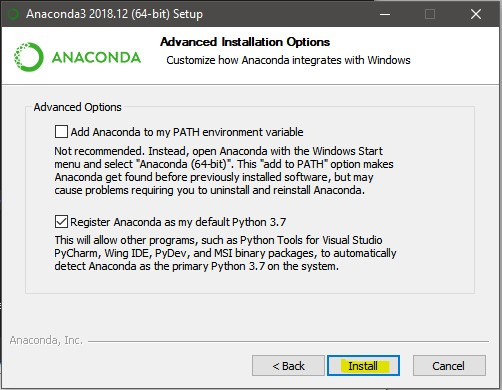
\includegraphics[height=3cm]{chapters/gambar/install5.jpg}
  \caption{Tampilan Instalasi 5}
\end{figure}

  \item Tunggu sampai instalasi selesai
\begin{figure}[!htbp]
  \centering
  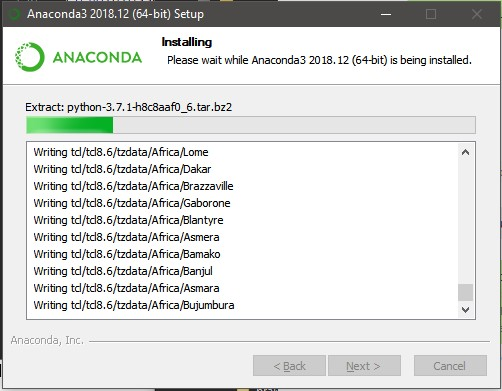
\includegraphics[height=3cm]{chapters/gambar/install6.jpg}
  \caption{Tampilan Instalasi 6}
\end{figure}

  \item Setelah selesai tekan 'Next'
\begin{figure}[!htbp]
  \centering
  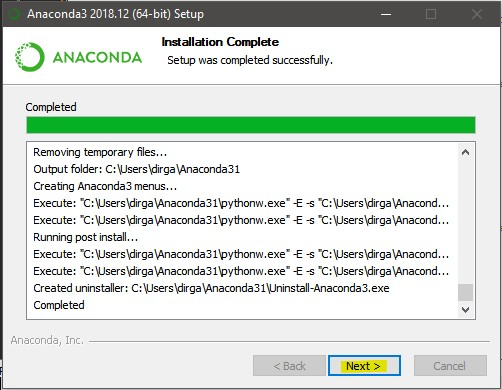
\includegraphics[height=3cm]{chapters/gambar/install7.jpg}
  \caption{Tampilan Instalasi 7}
\end{figure}

  \item Setelah itu ada opsi untuk memilih untuk meinstall visual studio code, jika anda berminat klik 'Install VSCode' jika tidak tekan 'Skip'
\begin{figure}[!htbp]
  \centering
  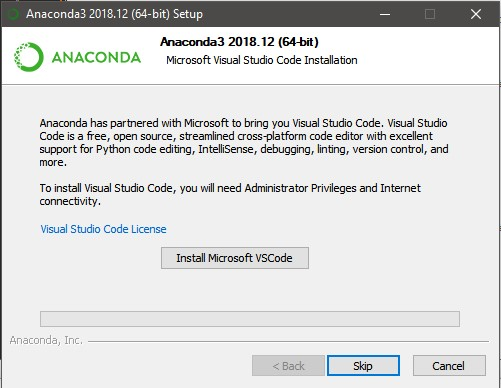
\includegraphics[height=3cm]{chapters/gambar/install8.jpg}
  \caption{Tampilan Instalasi 8}
\end{figure}

  \item Tekan 'Finish' untuk menyelesaikan instalasi
\begin{figure}[!htbp]
  \centering
  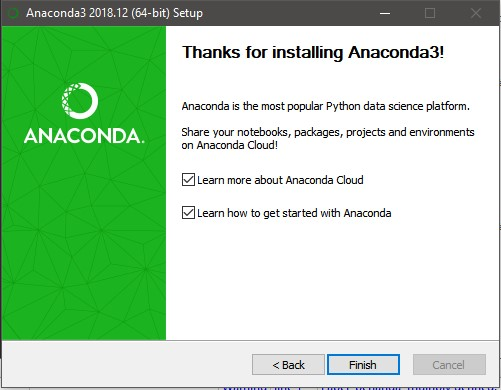
\includegraphics[height=3cm]{chapters/gambar/install9.jpg}
  \caption{Tampilan Instalasi 9}
\end{figure}

\end{enumerate}

\subsection{Cara menggunakan Spyder pada Anaconda}
Pertama buka aplikasi Anaconda sampai muncul seperti ini
\begin{figure}[!htbp]
  \centering
  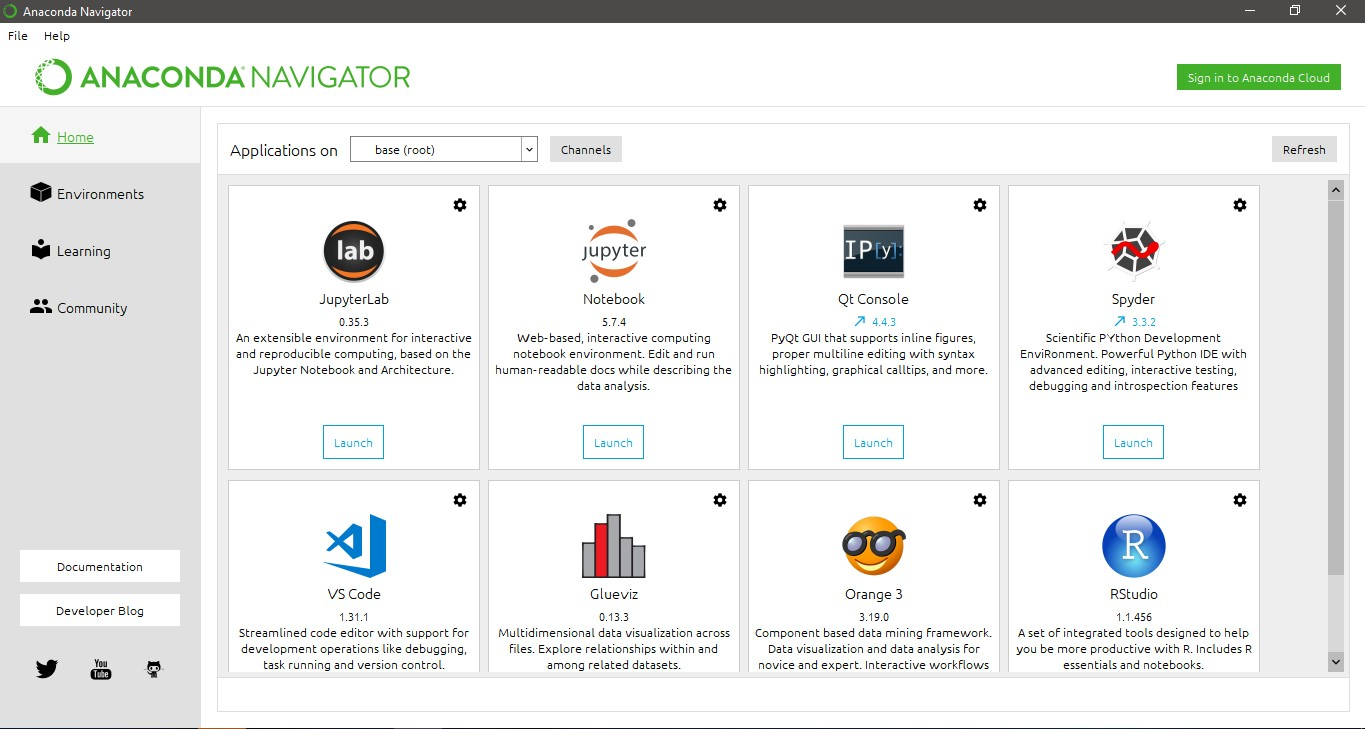
\includegraphics[height=3cm]{chapters/gambar/gambaranaconda.jpg}
  \caption{Tampilan awal Anaconda}
\end{figure}

Setelah itu tekan Launch dibawah logo Spyder
Tunggu sampai muncul seperti ini
\begin{figure}[!htbp]
  \centering
  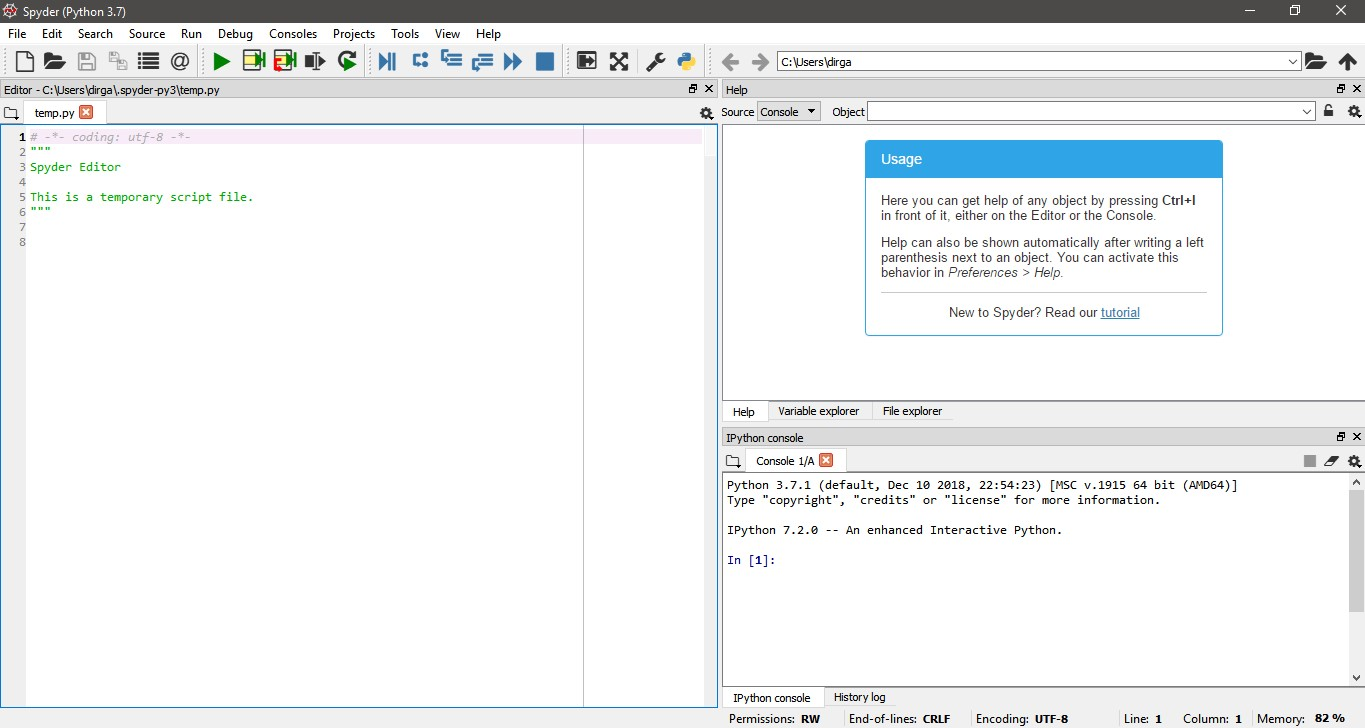
\includegraphics[height=3cm]{chapters/gambar/gambarspider.jpg}
  \caption{Tampilan spider}
\end{figure}

\subsection{Membuat Hello World di Spyder}
Setelah membuka spyder seperti gambar di section sebelumnya tekan menu File lalu klik New File atau bisa menggunakan kombinasi tombol Ctrl + N sampai muncul seperti ini

\begin{figure}[!htbp]
  \centering
  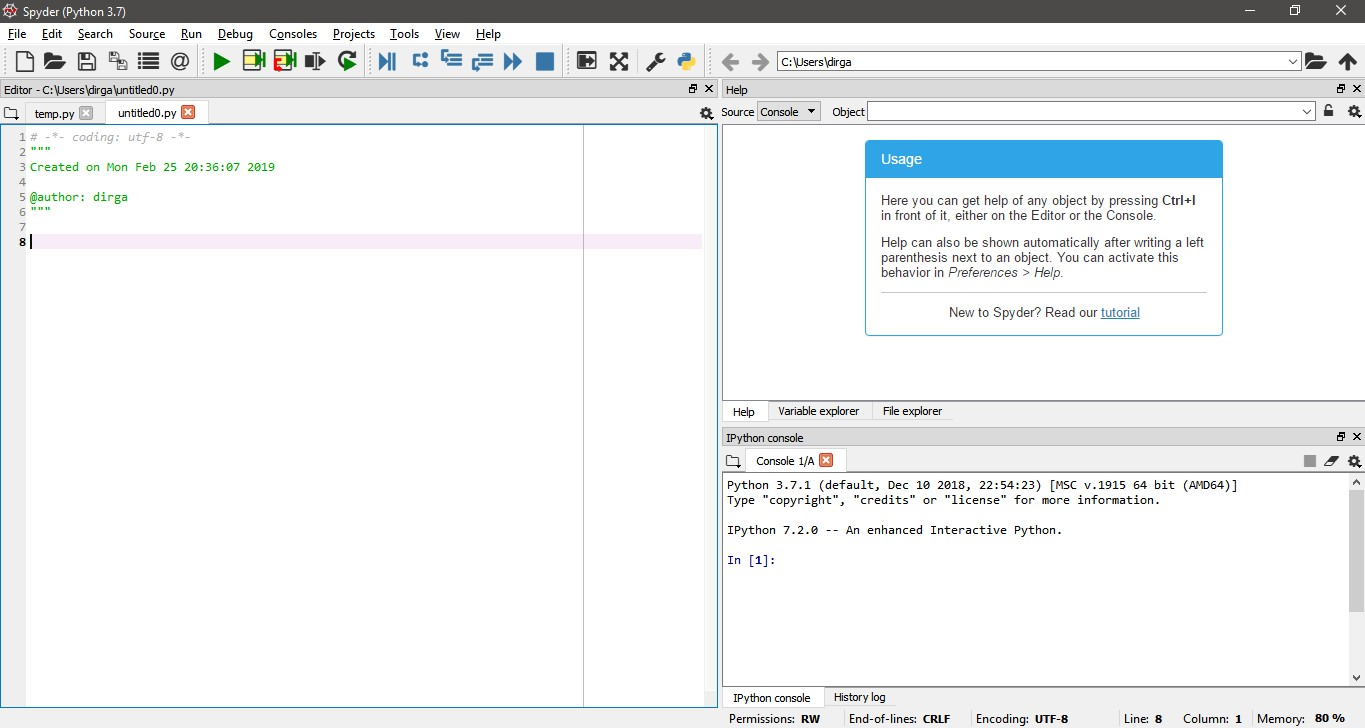
\includegraphics[height=3cm]{chapters/gambar/gambarnewfile.jpg}
  \caption{Tampilan new file pada spider}
\end{figure}

Karena kita menggunakan Python3.7 maka kita menggunakan funsi print() untuk memunculkan teks Hello World yang akan kita buat, tuliskan print("Hello World") pada teks editor di Spyder

\begin{figure}[!htbp]
  \centering
  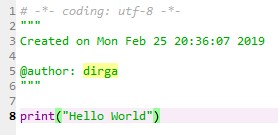
\includegraphics[height=3cm]{chapters/gambar/gambarprint.jpg}
  \caption{print("Hello World")}
\end{figure}

setelah itu tekan tombol play berwarna hijau diatas, karena kita belum save file yang kita buat maka akan muncul dialog simpan file, pilih tempat dan nama file yang akan disimpan contohnya helloworld.py

\begin{figure}[!htbp]
  \centering
  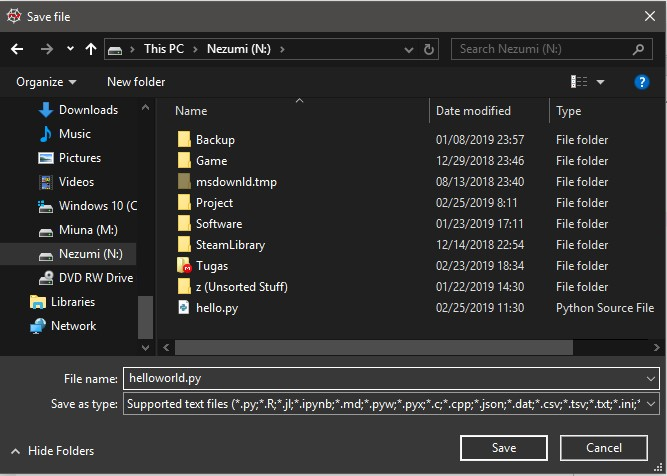
\includegraphics[height=3cm]{chapters/gambar/helloworld.jpg}
  \caption{Dialog simpan file}
\end{figure}

setelah itu tekan run maka hasil dari program yang kita buat tadi ada dibagian console yang berada di pinggir kanan bawah

\begin{figure}[!htbp]
  \centering
  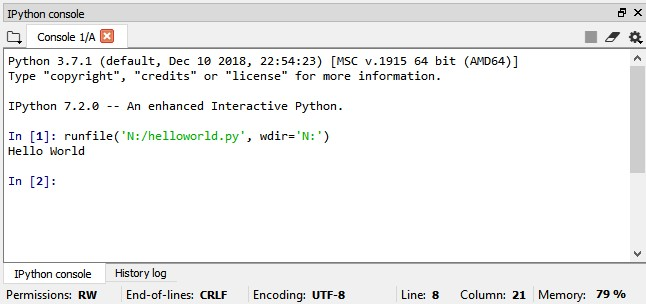
\includegraphics[height=3cm]{chapters/gambar/hasil.jpg}
  \caption{Hasil Program}
\end{figure}



\chapter{Chapter 2}
\section{Chapter 2 | D. Irga B. Naufal Fakhri D4 TI 2C}
\subsection{Teori Praktikum}
\begin{enumerate}
\item Jenis-jenis variabel pada python dan cara penggunaannya:

\begin{enumerate}
\item Boolean
\lstinputlisting[caption=Contoh kode variable Boolean., firstline=8, lastline=10]{src/1174066.py}

\item String
\lstinputlisting[caption=Contoh kode variable String., firstline=12, lastline=14]{src/1174066.py}

\item Integer
\lstinputlisting[caption=Contoh kode variable Integer., firstline=16, lastline=18]{src/1174066.py}

\item Float
\lstinputlisting[caption=Contoh kode variable Float., firstline=20, lastline=22]{src/1174066.py}

\item Hexadecimal
\lstinputlisting[caption=Contoh kode variable Hexadecimal., firstline=24, lastline=26]{src/1174066.py}

\item Complex
\lstinputlisting[caption=Contoh kode variable Complex., firstline=28, lastline=30]{src/1174066.py}

\item List
\lstinputlisting[caption=Contoh kode variable List., firstline=32, lastline=35]{src/1174066.py}

\item Tuple
\lstinputlisting[caption=Contoh kode variable Tuple., firstline=37, lastline=40]{src/1174066.py}

\item Set
\lstinputlisting[caption=Contoh kode variable Set., firstline=42, lastline=44]{src/1174066.py}

\item Dictionary
\lstinputlisting[caption=Contoh kode variable Dictionary., firstline=46, lastline=49]{src/1174066.py}

\end{enumerate}

\item Permintaan Input dari user dan Outputnya
\lstinputlisting[caption=Contoh kode input dan outputnya., firstline=51, lastline=53]{src/1174066.py}

\item Operator dasar aritmatika dan perubahan tipe data variable

Operator dasar aritmatika
\begin{enumerate}
\item Perjumlahan (+)
Operator ini berfungsi untuk melakukan operasi perjumlahan.
\lstinputlisting[caption=Contoh kode operasi pertambahan., firstline=51, lastline=60]{src/1174066.py}
\item Pengurangan (-)
Operator ini berfungsi untuk melakukan operasi pengurangan.
\lstinputlisting[caption=Contoh kode operasi pengurangan., firstline=62, lastline=66]{src/1174066.py}
\item Perkalian (*)
Operator ini dipergunakan untuk melakukan operasi perkalian.
\lstinputlisting[caption=Contoh kode operasi perkalian., firstline=68, lastline=72]{src/1174066.py}
\item Pembagian (/)
Operator ini dipergunakan untuk melakukan operasi pembagian.
\lstinputlisting[caption=Contoh kode operasi pembagian., firstline=74, lastline=78]{src/1174066.py}
\item Modulus (%)
Operator ini dipergunakan untuk melakukan operasi modulus.
\lstinputlisting[caption=Contoh kode operasi modulus., firstline=80, lastline=84]{src/1174066.py}
\item Perpangkatan (**)
Operator ini dipergunakan untuk melakukan operasi perpangkatan.
\lstinputlisting[caption=Contoh kode operasi perpangkatan., firstline=86, lastline=90]{src/1174066.py}
\item Pembulatan Kebawah Pada Hasil Pembagian (//)
Operator ini dipergunakan untuk melakukan operasi pembulatan hasil bagi.
\lstinputlisting[caption=Contoh kode operasi pembulatan hasil pembagian kebawah., firstline=92, lastline=96]{src/1174066.py}
\end{enumerate}

Perubahan tipe data variable
\begin{enumerate}
\item String menjadi Integer
\lstinputlisting[caption=Contoh kode variable string menjadi integer., firstline=99, lastline=102]{src/1174066.py}
\item Integer menjadi String
\lstinputlisting[caption=Contoh kode variable integer menjadi string., firstline=104, lastline=107]{src/1174066.py}
\end{enumerate}


\item Sintak perulangan (looping), jenis-jenisnya, dan penggunaannya.
\begin{enumerate}
\item While Loop
While Loop adalah perulangan yang mengeksekusi statement terus menerus selama kondisi bernilai True.
\lstinputlisting[caption=Contoh kode penggunaan while loop., firstline=111, lastline=115]{src/1174066.py}

\item For Loop
For Loop  adalah pengulangan berdasarkan kondisi yang telah ditentukan biasanya kondisi pertambahan seperti 1 sampai 5
\lstinputlisting[caption=Contoh kode penggunaan for loop., firstline=117, lastline=120]{src/1174066.py}

\item Nested Loop
Nested Loop merupakan pengulangan yang ada di dalam pengulangan
\lstinputlisting[caption=Contoh kode penggunaan nested loop., firstline=122, lastline=129]{src/1174066.py}

\end{enumerate}

\item Sintak kondisi dan penggunaannya.
\begin{enumerate}
\item If
Kondisi ini digunakan untuk mengecek apabila kondisi tersebut dipenuhi akan mengeksekusi kode didalamnya.
\lstinputlisting[caption=Contoh kode penggunaan if., firstline=132, lastline=136]{src/1174066.py}

\item If Else
Kondisi ini digunakan untuk mengecek apabila kondisi tersebut dipenuhi akan mengeksekusi kode didalamnya dan didalamnya memiliki dua kondisi.
\lstinputlisting[caption=Contoh kode penggunaan if else., firstline=138, lastline=143]{src/1174066.py}

\item Elif
Kondisi ini digunakan untuk mengecek apabila kondisi tersebut dipenuhi akan mengeksekusi kode didalamnya dan didalamnya memiliki dua kondisi atau lebih.
\lstinputlisting[caption=Contoh kode penggunaan elif., firstline=145, lastline=152]{src/1174066.py}

\item Kondisi di dalam kondisi
Kondisi ini digunakan saat kondisi memerlukan kondisi lagi didalamnya
\lstinputlisting[caption=Contoh kode penggunaan kondisi di dalam kondisi., firstline=155, lastline=165]{src/1174066.py}

\end{enumerate}

\item Jenis-jenis error pada python dan cara mengatasinya.
\begin{itemize}
\item Syntax Errors
Syntax Errors adalah kesalahan pada penulisan syntax atau kode. Solusinya adalah memperbaiki penulisan syntax atau kode

\item Zero Division Error
ZeroDivisonError adalah exceptions yang terjadi saat eksekusi program menghasilkan perhitungan matematika pembagian dengan angka nol (0). Solusinya adalah tidak membagi suatu yang hasilnya nol.

\item Name Error
NameError adalah exception saat kode melakukan eksekusi terhadap local name atau global name yang tidak terdefinisi atau tidak ada. Solusinya adalah memastikan variabel atau function yang akan dipanggil ada didalam program atau tidak salah mengetikannya.

\item Type Error
TypeError adalah exception saat melakukan eksekusi terhadap suatu operasi atau fungsi dengan type object yang tidak sesuai. Solusinya adalah mengkoversi varibelnya sesuai dengan tipe data sesuai dengan yang akan digunakan.

\end{itemize}

\item Cara pemakaian Try Except.
\lstinputlisting[caption=Contoh kode penggunaan try except., firstline=168, lastline=174]{src/1174066.py}

\end{enumerate}
\hfill \break

\subsection{Ketrampilan Pemrograman}

\begin{enumerate}
\item Jawaban Soal 1
\lstinputlisting[firstline=117, lastline=200]{src/1174066.py}

\item Jawaban Soal 2
\lstinputlisting[firstline=203, lastline=209]{src/1174066.py}

\item Jawaban Soal 3
\lstinputlisting[firstline=212, lastline=219]{src/1174066.py}

\item Jawaban Soal 4
\lstinputlisting[firstline=222, lastline=225]{src/1174066.py}

\item Jawaban Soal 5
\lstinputlisting[firstline=228, lastline=242]{src/1174066.py}

\item Jawaban Soal 6
\lstinputlisting[firstline=245, lastline=247]{src/1174066.py}

\item Jawaban Soal 7
\lstinputlisting[firstline=250, lastline=252]{src/1174066.py}

\item Jawaban Soal 8
\lstinputlisting[firstline=255, lastline=258]{src/1174066.py}

\item Jawaban Soal 9
\lstinputlisting[firstline=261, lastline=268]{src/1174066.py}

\item Jawaban Soal 10
\lstinputlisting[firstline=271, lastline=277]{src/1174066.py}

\item Jawaban Soal 11
\lstinputlisting[firstline=280, lastline=288]{src/1174066.py}

\end{enumerate}
\hfill \break

\subsection{Ketrampilan Penanganan Error}
\begin{enumerate}
\item Jawaban Soal No. 1
\begin{itemize}
\item Syntax Errors
Syntax Errors adalah kesalahan pada penulisan syntax atau kode. Solusinya adalah memperbaiki penulisan syntax atau kode

\item Zero Division Error
ZeroDivisonError adalah exceptions yang terjadi saat eksekusi program menghasilkan perhitungan matematika pembagian dengan angka nol (0). Solusinya adalah tidak membagi suatu yang hasilnya nol.

\item Name Error
NameError adalah exception saat kode melakukan eksekusi terhadap local name atau global name yang tidak terdefinisi atau tidak ada. Solusinya adalah memastikan variabel atau function yang akan dipanggil ada didalam program atau tidak salah mengetikannya.

\item Type Error
TypeError adalah exception saat melakukan eksekusi terhadap suatu operasi atau fungsi dengan type object yang tidak sesuai. Solusinya adalah mengkoversi varibelnya sesuai dengan tipe data sesuai dengan yang akan digunakan.

\end{itemize}

\item Jawaban Soal No. 2																			
\lstinputlisting[firstline=1, lastline=7]{src/2err_1174066.py}
\end{enumerate}



\bibliographystyle{IEEEtran} 
%\def\bibfont{\normalsize}
\bibliography{references}


%%%%%%%%%%%%%%%
%%  The default LaTeX Index
%%  Don't need to add any commands before \begin{document}
\printindex

%%%% Making an index
%% 
%% 1. Make index entries, don't leave any spaces so that they
%% will be sorted correctly.
%% 
%% \index{term}
%% \index{term!subterm}
%% \index{term!subterm!subsubterm}
%% 
%% 2. Run LaTeX several times to produce <filename>.idx
%% 
%% 3. On command line, type  makeindx <filename> which
%% will produce <filename>.ind 
%% 
%% 4. Type \printindex to make the index appear in your book.
%% 
%% 5. If you would like to edit <filename>.ind 
%% you may do so. See docs.pdf for more information.
%% 
%%%%%%%%%%%%%%%%%%%%%%%%%%%%%%

%%%%%%%%%%%%%% Making Multiple Indices %%%%%%%%%%%%%%%%
%% 1. 
%% \usepackage{multind}
%% \makeindex{book}
%% \makeindex{authors}
%% \begin{document}
%% 
%% 2.
%% % add index terms to your book, ie,
%% \index{book}{A term to go to the topic index}
%% \index{authors}{Put this author in the author index}
%% 
%% \index{book}{Cows}
%% \index{book}{Cows!Jersey}
%% \index{book}{Cows!Jersey!Brown}
%% 
%% \index{author}{Douglas Adams}
%% \index{author}{Boethius}
%% \index{author}{Mark Twain}
%% 
%% 3. On command line type 
%% makeindex topic 
%% makeindex authors
%% 
%% 4.
%% this is a Wiley command to make the indices print:
%% \multiprintindex{book}{Topic index}
%% \multiprintindex{authors}{Author index}

\end{document}

